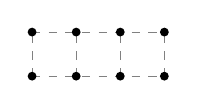
\begin{tikzpicture}[scale = 0.56]
  \draw[dashed,gray] (0,0) grid (3,1);
  \foreach \x in {0,1,2,3} {
    \fill (\x, 0) circle (0.1);
    \fill (\x, 1) circle (0.1);
  }
\end{tikzpicture}
~
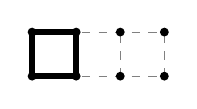
\begin{tikzpicture}[scale = 0.56]
  \draw[dashed,gray] (0,0) grid (3,1);
  \draw[line width = 2] (0,0) rectangle (1,1);
  \foreach \x in {0,1,2,3} {
    \fill (\x, 0) circle (0.1);
    \fill (\x, 1) circle (0.1);
  }
\end{tikzpicture}
~
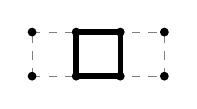
\begin{tikzpicture}[scale = 0.56]
  \draw[dashed,gray] (0,0) grid (3,1);
  \draw[line width = 2] (1,0) rectangle (2,1);
  \foreach \x in {0,1,2,3} {
    \fill (\x, 0) circle (0.1);
    \fill (\x, 1) circle (0.1);
  }
\end{tikzpicture}
~

\begin{tikzpicture}[scale = 0.56]
  \draw[dashed,gray] (0,0) grid (3,1);
  \draw[line width = 2] (0,0) rectangle (1,1) (2,0) rectangle (3,1);
  \foreach \x in {0,1,2,3} {
    \fill (\x, 0) circle (0.1);
    \fill (\x, 1) circle (0.1);
  }
\end{tikzpicture}
~
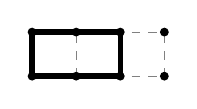
\begin{tikzpicture}[scale = 0.56]
  \draw[dashed,gray] (0,0) grid (3,1);
  \draw[line width = 2] (0,0) rectangle (2,1);
  \foreach \x in {0,1,2,3} {
    \fill (\x, 0) circle (0.1);
    \fill (\x, 1) circle (0.1);
  }
\end{tikzpicture}
\\~\\
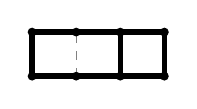
\begin{tikzpicture}[scale = 0.56]
  \draw[dashed,gray] (0,0) grid (3,1);
  \draw[line width = 2] (0,0) rectangle (2,1) rectangle (3,0);
  \foreach \x in {0,1,2,3} {
    \fill (\x, 0) circle (0.1);
    \fill (\x, 1) circle (0.1);
  }
\end{tikzpicture}
~
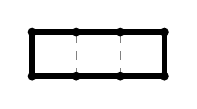
\begin{tikzpicture}[scale = 0.56]
  \draw[dashed,gray] (0,0) grid (3,1);
  \draw[line width = 2] (0,0) rectangle (3,1);
  \foreach \x in {0,1,2,3} {
    \fill (\x, 0) circle (0.1);
    \fill (\x, 1) circle (0.1);
  }
\end{tikzpicture}
~
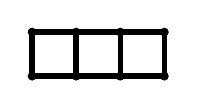
\begin{tikzpicture}[scale = 0.56]
  \draw[dashed,gray] (0,0) grid (3,1);
  \draw[line width = 2] (0,0) rectangle (1,1) rectangle (2,0) rectangle (3,1);
  \foreach \x in {0,1,2,3} {
    \fill (\x, 0) circle (0.1);
    \fill (\x, 1) circle (0.1);
  }
\end{tikzpicture}
~

\begin{tikzpicture}[scale = 0.56]
  \draw[dashed,gray] (0,0) grid (3,1);
  \draw[line width = 2] (0,0) rectangle (1,1)--(2,1) rectangle (3,0);
  \foreach \x in {0,1,2,3} {
    \fill (\x, 0) circle (0.1);
    \fill (\x, 1) circle (0.1);
  }
\end{tikzpicture}
~
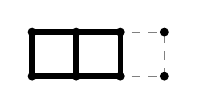
\begin{tikzpicture}[scale = 0.56]
  \draw[dashed,gray] (0,0) grid (3,1);
  \draw[line width = 2] (0,0) rectangle (1,1) rectangle (2,0);
  \foreach \x in {0,1,2,3} {
    \fill (\x, 0) circle (0.1);
    \fill (\x, 1) circle (0.1);
  }
\end{tikzpicture}